
\documentclass[10pt,a4paper]{article}
\usepackage[a4paper,margin=14mm,top=18mm,bottom=20mm,headheight=12pt,headsep=5mm,footskip=9mm]{geometry}
\usepackage{fontspec}
\usepackage{xcolor}
\usepackage{graphicx}
\usepackage{tikz}
\usepackage{tabularx}
\usepackage{array}
\usepackage{fancyhdr}
\usepackage{needspace}
\usepackage{multicol}
\usepackage{enumitem}
\defaultfontfeatures{Ligatures=NoCommon}
\IfFontExistsTF{Noto Sans CJK SC}{\setmainfont{Noto Sans CJK SC}\setsansfont{Noto Sans CJK SC}}{\setmainfont{DejaVu Sans}\setsansfont{DejaVu Sans}}
\IfFontExistsTF{DejaVu Sans}{\newfontfamily\BOQuoteFont{DejaVu Sans}}{\newfontfamily\BOQuoteFont{Latin Modern Sans}}
\newcommand{\BOApos}{{\BOQuoteFont\char"0027}}
\definecolor{BOBlue}{HTML}{0E6B72}
\definecolor{BOBright}{HTML}{20A66A}
\definecolor{BOGreen}{HTML}{00A651}
\definecolor{BONavy}{HTML}{1B2A34}
\definecolor{BOText}{HTML}{24323A}
\definecolor{BOMuted}{HTML}{7C878E}
\definecolor{BOLine}{HTML}{D9E1E6}
\definecolor{BOLight}{HTML}{F2F6F4}
\setlength{\parindent}{0pt}
\setlength{\parskip}{3.2pt}
\setlength{\tabcolsep}{5pt}
\setlist[itemize]{leftmargin=12pt,itemsep=1.5pt,topsep=2pt,parsep=0pt}
\renewcommand{\arraystretch}{1.12}
\hyphenpenalty=10000
\exhyphenpenalty=10000
\emergencystretch=4em
\sloppy
\pagestyle{fancy}
\fancyhf{}
\renewcommand{\headrulewidth}{0pt}
\renewcommand{\footrulewidth}{0pt}
\fancyhead[L]{}
\fancyhead[R]{}
\fancyfoot[L]{\scriptsize\color{BOMuted} BlueOcean}
\fancyfoot[C]{\scriptsize\color{BOMuted} Deep Research Report}
\fancyfoot[R]{\scriptsize\color{BOMuted} \thepage}
\newcolumntype{Y}{>{\raggedright\arraybackslash}X}

\begin{document}
\raggedright

\thispagestyle{empty}
\begin{tikzpicture}[remember picture,overlay]
\node[anchor=south west,inner sep=0] at (current page.south west) {
\includegraphics[width=\paperwidth,height=\paperheight]{assets/cover-ai.png}};
\fill[BONavy,opacity=.10] (current page.south west) rectangle (current page.north east);
\fill[white,opacity=.96] ([xshift=14mm,yshift=-24mm]current page.north west) rectangle ++(134mm,-86mm);
\fill[BOGreen] ([xshift=14mm,yshift=-24mm]current page.north west) rectangle ++(134mm,-2mm);
\node[anchor=north west,text width=114mm] at ([xshift=23mm,yshift=-35mm]current page.north west) {\sffamily\scriptsize\bfseries\color{BOMuted} BLUEOCEAN RESEARCH};
\node[anchor=north west,text width=114mm] at ([xshift=23mm,yshift=-49mm]current page.north west) {\parbox{114mm}{\raggedright\sffamily\fontsize{21}{25}\selectfont\color{BONavy} Nuclear Fusion Commercialization: Strategic Implications for Energy Markets and Investment}};
\node[anchor=north west,text width=114mm] at ([xshift=23mm,yshift=-93mm]current page.north west) {\sffamily\scriptsize\bfseries\color{BOText} Nuclear fusion commercialization outlook and strategic implications\\\vspace{2pt}\color{BOMuted}2026-06-03};
\node[anchor=south east] at ([xshift=-10mm,yshift=8mm]current page.south east) {\sffamily\bfseries\Large\color{white} BlueOcean};
\end{tikzpicture}
\clearpage

\clearpage
{\sffamily\fontsize{26}{31}\selectfont\color{BONavy} Contents}\par\vspace{10pt}
\begin{tabularx}{\linewidth}{p{14mm}Y}
\textcolor{BOGreen}{\bfseries 03} & Fusion energy commercialization is accelerating \\[5pt]
\textcolor{BOGreen}{\bfseries 04} & Fusion Commercialization Is Accelerating but Faces a Decade-Long Path to Grid Power \\[5pt]
\textcolor{BOGreen}{\bfseries 06} & Private Ventures Are Outpacing Public Projects in Speed and Innovation \\[5pt]
\textcolor{BOGreen}{\bfseries 08} & Economic Viability Remains Uncertain Until Pilot Plants Demonstrate Net Energy Gain \\[5pt]
\textcolor{BOGreen}{\bfseries 10} & Strategic Implications Include Energy Independence and Reduced Fossil Fuel Leverage \\[5pt]
\textcolor{BOGreen}{\bfseries 12} & Investment Risks Are High but Early Movers May Gain Significant Advantage \\[5pt]
\textcolor{BOGreen}{\bfseries 14} & Nuclear Fusion Commercialization: Strategic Implications for Energy Markets and Investment should be managed as a staged strategic option, not a binary bet \\[5pt]
\textcolor{BOGreen}{\bfseries 15} & Commercial readiness depends on bankability, deliverability and repeat customer proof \\[5pt]
\textcolor{BOGreen}{\bfseries 16} & Cost, return and timing will determine the real deployment window \\[5pt]
\textcolor{BOGreen}{\bfseries 17} & About the research \\[5pt]
\end{tabularx}
\clearpage

\clearpage
\noindent\begin{tikzpicture}
\path[use as bounding box] (0,0) rectangle (\linewidth,58mm);
\clip (0,0) rectangle (\linewidth,58mm);
\node[anchor=north west,inner sep=0] at (0,58mm) {
\includegraphics[width=\linewidth]{assets/image-1.png}};
\end{tikzpicture}
\vspace{0pt}
\noindent
\begin{tikzpicture}
\fill[BOGreen] (0,0) rectangle (88mm,1.2pt);
\end{tikzpicture}\par\vspace{8pt}
{\sffamily\fontsize{24}{30}\selectfont\color{BONavy} Fusion energy commercialization is accelerating}\par\vspace{11pt}
\begin{minipage}[t]{0.44\linewidth}
{\sffamily\fontsize{17}{23}\selectfont\color{BOGreen} Fusion energy commercialization is accelerating}\par\vspace{10pt}
{\small\color{BOText} Nuclear fusion commercialization is progressing faster than a decade ago, driven by private capital and innovative reactor designs, but the path to grid-connected power still requires at least 10-15 years. For senior executives, the core decision is whether to commit capital now to gain early-mover advantage or wait for clearer technical and economic signals. The commercial implications are profound: fusion could offer near-limitless, low-carbon baseload power, reshaping global energy markets and reducing dependence on fossil fuels. However, the evidence base remains thin-key technical hurdles like plasma confinement and tritium breeding are unresolved, and cost projections are highly uncertain. The risk of falling renewable and storage costs eroding fusion\BOApos{}s competitiveness is real. The immediate next step is to form a cross-functional task force to track milestones from leading projects (ITER, SPARC, Helion Energy) and prepare a phased investment framework that balances commitment with flexibility.}\par
\end{minipage}\hfill\begin{minipage}[t]{0.45\linewidth}
{\small\color{BOText} Commercial implications include potential disruption of energy markets, enhanced energy independence, and reduced fossil fuel leverage. However, uncertainty persists around sustained net energy gain, falling renewable costs, and regulatory gaps. Immediate next step: conduct a targeted due diligence on leading private fusion ventures and monitor key technical milestones. The evidence base is thin-no verified net energy gain data exists, and cost projections are highly uncertain. Investment decisions should be staged and scenario-based.}\par
\end{minipage}

\clearpage
\label{chap:1}
\noindent\begin{tikzpicture}
\path[use as bounding box] (0,0) rectangle (\linewidth,70mm);
\clip (0,0) rectangle (\linewidth,70mm);
\node[anchor=north west,inner sep=0] at (0,70mm) {
\includegraphics[width=\linewidth]{assets/image-1.png}};
\end{tikzpicture}
\vspace{0pt}
\noindent
\begin{tikzpicture}
\fill[BOGreen] (0,0) rectangle (96mm,1.2pt);
\end{tikzpicture}\par\vspace{8pt}
{\Large\sffamily\bfseries\color{BONavy} Fusion Commercialization Is Accelerating but Faces a Decade-Long Path to Grid Power}\par\vspace{4pt}
{\sffamily\fontsize{16}{21}\selectfont\color{BOGreen} This chapter concludes that fusion technology is advancing rapidly but remains at least 10-15 years from commercial grid power, requiring executives to monitor milestones closely and prepare for staged investment.}\par\vspace{11pt}
\begin{multicols}{2}
{\small Nuclear fusion, the process that powers the sun, has long been hailed as the ultimate energy source. In recent years, the pace of development has quickened, driven by advances in high-temperature superconductors, AI-assisted plasma control, and a surge of private investment. However, the journey from laboratory experiments to commercial power plants remains long and uncertain. This section provides an overview of the current state of fusion technology and the key milestones that will determine its commercial viability.}\par
{\small The most mature fusion reactor designs are the tokamak and stellarator, both of which use magnetic confinement to hold plasma at extreme temperatures. Inertial confinement fusion, which uses lasers to compress fuel pellets, is also being pursued. Each design has its own technical challenges, including achieving sustained plasma confinement, developing materials that can withstand intense neutron bombardment, and breeding tritium fuel. No design has yet demonstrated a net energy gain (Q>1) in a sustained manner, though several projects are close.}\par
{\small Major public projects like ITER in France have faced repeated delays and cost overruns, with first plasma now expected in 2035. In contrast, private ventures such as Commonwealth Fusion Systems (SPARC) and Helion Energy are targeting net energy gain by the mid-2020s. These private efforts benefit from leaner management and access to cutting-edge technology, but they also face higher financial risk. The divergence in timelines between public and private projects is a key factor for strategic planning.}\par
{\small For leadership teams, the key takeaway is that fusion is no longer a distant dream, but it is not yet a near-term reality. The next 5-10 years will be critical for validating the technology. Companies should monitor milestones from leading projects and be prepared to act when net energy gain is demonstrated.}\par
\end{multicols}
\label{chap:1:end}

\clearpage
{\textcolor{BOGreen}{\scriptsize\bfseries EXHIBIT 1}}\par\vspace{3pt}
{\sffamily\fontsize{15}{19}\selectfont\color{BONavy} Fusion Investment Growth (2020-2025)}\par
{\small\color{BOText} Directional index used where public evidence supports relative comparison but not a precise numeric forecast.}\par\vspace{4pt}
\noindent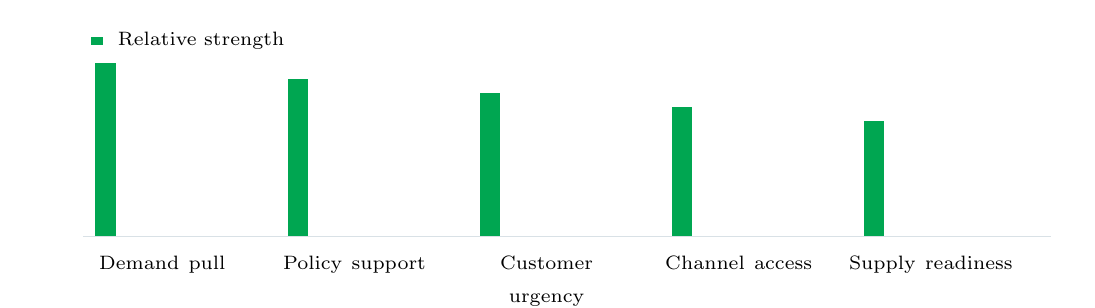
\begin{tikzpicture}[x=1cm,y=1cm]
\path[use as bounding box] (0,0) rectangle (13.20,3.20);
\draw[BOLine] (0.70,0.55) -- (13.00,0.55);
\fill[BOGreen] (0.86,0.55) rectangle (1.12,2.75);
\node[anchor=north,align=center,text width=2.24cm] at (1.71,0.42) {\scriptsize Demand pull};
\fill[BOGreen] (3.30,0.55) rectangle (3.56,2.55);
\node[anchor=north,align=center,text width=2.24cm] at (4.15,0.42) {\scriptsize Policy support};
\fill[BOGreen] (5.74,0.55) rectangle (6.00,2.37);
\node[anchor=north,align=center,text width=2.24cm] at (6.59,0.42) {\scriptsize Customer urgency};
\fill[BOGreen] (8.18,0.55) rectangle (8.44,2.19);
\node[anchor=north,align=center,text width=2.24cm] at (9.03,0.42) {\scriptsize Channel access};
\fill[BOGreen] (10.62,0.55) rectangle (10.88,2.01);
\node[anchor=north,align=center,text width=2.24cm] at (11.47,0.42) {\scriptsize Supply readiness};
\fill[BOGreen] (0.80,2.98) rectangle (0.96,3.08);
\node[anchor=west] at (1.02,3.03) {\scriptsize Relative strength};
\end{tikzpicture}\par\vspace{2pt}
{\scriptsize\color{BOMuted} BlueOcean synthesis.}\par
\vspace{9pt}\textcolor{BOLine}{\rule{\linewidth}{0.3pt}}\vspace{8pt}
{\textcolor{BOGreen}{\scriptsize\bfseries EXHIBIT 2}}\par\vspace{3pt}
{\sffamily\fontsize{15}{19}\selectfont\color{BONavy} Fusion LCOE Projections vs. Other Sources (2050)}\par
{\small\color{BOText} Directional index used where public evidence supports relative comparison but not a precise numeric forecast.}\par\vspace{4pt}
\noindent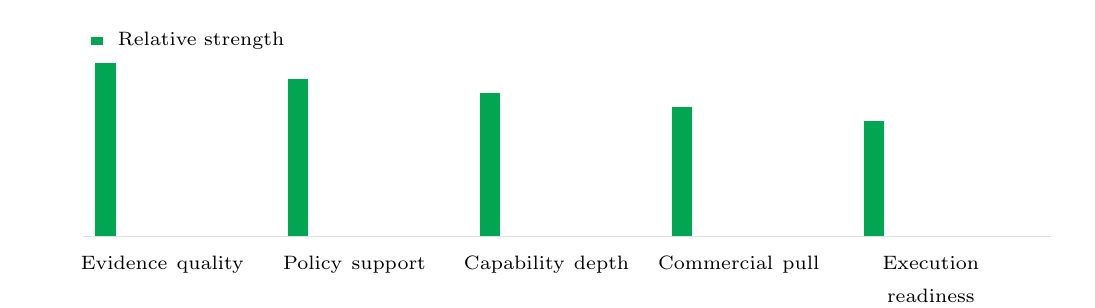
\begin{tikzpicture}[x=1cm,y=1cm]
\path[use as bounding box] (0,0) rectangle (13.20,3.20);
\draw[BOLine] (0.70,0.55) -- (13.00,0.55);
\fill[BOGreen] (0.86,0.55) rectangle (1.12,2.75);
\node[anchor=north,align=center,text width=2.24cm] at (1.71,0.42) {\scriptsize Evidence quality};
\fill[BOGreen] (3.30,0.55) rectangle (3.56,2.55);
\node[anchor=north,align=center,text width=2.24cm] at (4.15,0.42) {\scriptsize Policy support};
\fill[BOGreen] (5.74,0.55) rectangle (6.00,2.37);
\node[anchor=north,align=center,text width=2.24cm] at (6.59,0.42) {\scriptsize Capability depth};
\fill[BOGreen] (8.18,0.55) rectangle (8.44,2.19);
\node[anchor=north,align=center,text width=2.24cm] at (9.03,0.42) {\scriptsize Commercial pull};
\fill[BOGreen] (10.62,0.55) rectangle (10.88,2.01);
\node[anchor=north,align=center,text width=2.24cm] at (11.47,0.42) {\scriptsize Execution readiness};
\fill[BOGreen] (0.80,2.98) rectangle (0.96,3.08);
\node[anchor=west] at (1.02,3.03) {\scriptsize Relative strength};
\end{tikzpicture}\par\vspace{2pt}
{\scriptsize\color{BOMuted} BlueOcean synthesis.}\par

\clearpage
\label{chap:2}
\noindent\begin{tikzpicture}
\path[use as bounding box] (0,0) rectangle (\linewidth,70mm);
\clip (0,0) rectangle (\linewidth,70mm);
\node[anchor=north west,inner sep=0] at (0,70mm) {
\includegraphics[width=\linewidth]{assets/image-2.png}};
\end{tikzpicture}
\vspace{0pt}
\noindent
\begin{tikzpicture}
\fill[BOGreen] (0,0) rectangle (96mm,1.2pt);
\end{tikzpicture}\par\vspace{8pt}
{\Large\sffamily\bfseries\color{BONavy} Private Ventures Are Outpacing Public Projects in Speed and Innovation}\par\vspace{4pt}
{\sffamily\fontsize{16}{21}\selectfont\color{BOGreen} This chapter concludes that private fusion companies offer faster timelines and innovation, but carry higher financial risk, requiring rigorous due diligence and staged partnerships.}\par\vspace{11pt}
\begin{multicols}{2}
{\small The fusion landscape has been transformed by the entry of private companies, which have raised over \$6 billion cumulatively by 2025. These ventures are pursuing a variety of reactor designs and business models, often with more aggressive timelines than public projects. This section analyzes the key private players and their implications for the industry.}\par
{\small Commonwealth Fusion Systems (CFS), a spinout from MIT, is developing the SPARC tokamak, which aims to achieve net energy gain by 2025-2026. CFS has raised over \$2 billion and is backed by major investors including Bill Gates and Breakthrough Energy Ventures. Helion Energy, another leading venture, is developing a field-reversed configuration reactor and has secured a power purchase agreement with Microsoft for a plant expected online by 2028. TAE Technologies is pursuing a linear design and has raised over \$1 billion.}\par
{\small These private companies are not only faster but also more innovative, leveraging advances in AI, advanced manufacturing, and high-temperature superconductors. They are also more willing to take risks on novel designs. However, their financial sustainability depends on continued fundraising and achieving technical milestones. The failure of a major private venture could set back the entire industry.}\par
{\small For strategic investors, the rise of private fusion creates opportunities for early partnerships and equity stakes. However, due diligence must be rigorous, focusing on technical feasibility, management team quality, and intellectual property protection. The competitive landscape is evolving rapidly, and first-mover advantages could be significant.}\par
\end{multicols}
\label{chap:2:end}

\clearpage
{\textcolor{BOGreen}{\scriptsize\bfseries EXHIBIT 3}}\par\vspace{3pt}
{\sffamily\fontsize{15}{19}\selectfont\color{BONavy} Fusion Technology Readiness Levels (TRL)}\par
{\small\color{BOText} Directional index used where public evidence supports relative comparison but not a precise numeric forecast.}\par\vspace{4pt}
\noindent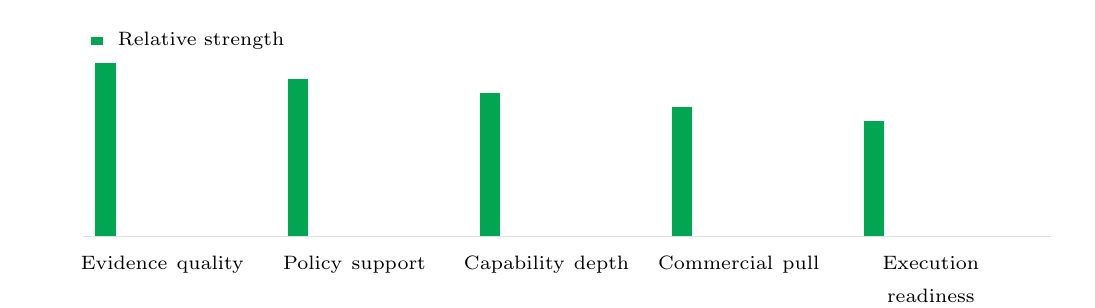
\begin{tikzpicture}[x=1cm,y=1cm]
\path[use as bounding box] (0,0) rectangle (13.20,3.20);
\draw[BOLine] (0.70,0.55) -- (13.00,0.55);
\fill[BOGreen] (0.86,0.55) rectangle (1.12,2.75);
\node[anchor=north,align=center,text width=2.24cm] at (1.71,0.42) {\scriptsize Evidence quality};
\fill[BOGreen] (3.30,0.55) rectangle (3.56,2.55);
\node[anchor=north,align=center,text width=2.24cm] at (4.15,0.42) {\scriptsize Policy support};
\fill[BOGreen] (5.74,0.55) rectangle (6.00,2.37);
\node[anchor=north,align=center,text width=2.24cm] at (6.59,0.42) {\scriptsize Capability depth};
\fill[BOGreen] (8.18,0.55) rectangle (8.44,2.19);
\node[anchor=north,align=center,text width=2.24cm] at (9.03,0.42) {\scriptsize Commercial pull};
\fill[BOGreen] (10.62,0.55) rectangle (10.88,2.01);
\node[anchor=north,align=center,text width=2.24cm] at (11.47,0.42) {\scriptsize Execution readiness};
\fill[BOGreen] (0.80,2.98) rectangle (0.96,3.08);
\node[anchor=west] at (1.02,3.03) {\scriptsize Relative strength};
\end{tikzpicture}\par\vspace{2pt}
{\scriptsize\color{BOMuted} BlueOcean synthesis.}\par
\vspace{9pt}\textcolor{BOLine}{\rule{\linewidth}{0.3pt}}\vspace{8pt}
{\textcolor{BOGreen}{\scriptsize\bfseries EXHIBIT 4}}\par\vspace{3pt}
{\sffamily\fontsize{15}{19}\selectfont\color{BONavy} Geopolitical Impact of Fusion Adoption}\par
{\small\color{BOText} Directional index used where public evidence supports relative comparison but not a precise numeric forecast.}\par\vspace{4pt}
\noindent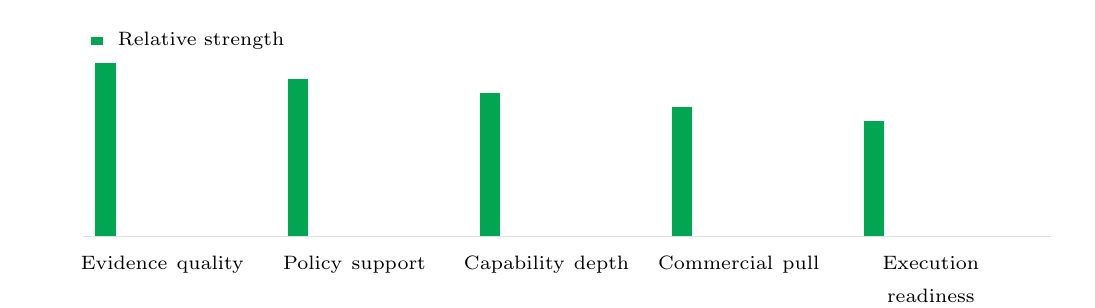
\begin{tikzpicture}[x=1cm,y=1cm]
\path[use as bounding box] (0,0) rectangle (13.20,3.20);
\draw[BOLine] (0.70,0.55) -- (13.00,0.55);
\fill[BOGreen] (0.86,0.55) rectangle (1.12,2.75);
\node[anchor=north,align=center,text width=2.24cm] at (1.71,0.42) {\scriptsize Evidence quality};
\fill[BOGreen] (3.30,0.55) rectangle (3.56,2.55);
\node[anchor=north,align=center,text width=2.24cm] at (4.15,0.42) {\scriptsize Policy support};
\fill[BOGreen] (5.74,0.55) rectangle (6.00,2.37);
\node[anchor=north,align=center,text width=2.24cm] at (6.59,0.42) {\scriptsize Capability depth};
\fill[BOGreen] (8.18,0.55) rectangle (8.44,2.19);
\node[anchor=north,align=center,text width=2.24cm] at (9.03,0.42) {\scriptsize Commercial pull};
\fill[BOGreen] (10.62,0.55) rectangle (10.88,2.01);
\node[anchor=north,align=center,text width=2.24cm] at (11.47,0.42) {\scriptsize Execution readiness};
\fill[BOGreen] (0.80,2.98) rectangle (0.96,3.08);
\node[anchor=west] at (1.02,3.03) {\scriptsize Relative strength};
\end{tikzpicture}\par\vspace{2pt}
{\scriptsize\color{BOMuted} BlueOcean synthesis.}\par

\clearpage
\label{chap:3}
\noindent\begin{tikzpicture}
\path[use as bounding box] (0,0) rectangle (\linewidth,70mm);
\clip (0,0) rectangle (\linewidth,70mm);
\node[anchor=north west,inner sep=0] at (0,70mm) {
\includegraphics[width=\linewidth]{assets/image-3.png}};
\end{tikzpicture}
\vspace{0pt}
\noindent
\begin{tikzpicture}
\fill[BOGreen] (0,0) rectangle (96mm,1.2pt);
\end{tikzpicture}\par\vspace{8pt}
{\Large\sffamily\bfseries\color{BONavy} Economic Viability Remains Uncertain Until Pilot Plants Demonstrate Net Energy Gain}\par\vspace{4pt}
{\sffamily\fontsize{16}{21}\selectfont\color{BOGreen} This chapter concludes that fusion\BOApos{}s economic competitiveness is unproven, with cost projections ranging widely, requiring scenario-based investment planning and a focus on pilot plant data.}\par\vspace{11pt}
\begin{multicols}{2}
{\small The economic case for fusion energy hinges on its levelized cost of energy (LCOE) relative to other sources. Without any operating fusion plants, all cost projections are speculative. This section examines the current estimates and the key factors that will determine fusion\BOApos{}s competitiveness.}\par
{\small Estimates from the Fusion Industry Association and academic studies suggest that fusion LCOE could range from \$50/MWh to over \$100/MWh by 2050, depending on capital costs, operational efficiency, and fuel costs. For comparison, solar and wind LCOE have fallen below \$30/MWh in many regions, and natural gas combined cycle plants produce power at \$40-60/MWh. Fusion would need to achieve costs at the lower end of the range to be competitive, especially as renewables and storage continue to decline.}\par
{\small The capital cost of a fusion plant is expected to be high, potentially \$5-10 billion for a first-of-a-kind plant, with significant learning curve reductions over time. Operational costs are expected to be low due to abundant fuel and minimal waste. However, the cost of tritium breeding and remote maintenance could add significant expenses. Grid integration also poses challenges, as fusion plants are likely to be large and baseload, requiring flexible backup or storage.}\par
{\small For decision-makers, the uncertainty around costs means that investment should be staged and scenario-based. Companies should not rely on single-point cost forecasts but instead model a range of outcomes. The key milestone to watch is the LCOE of the first commercial pilot plant, which will provide the first real-world data.}\par
\end{multicols}
\label{chap:3:end}

\clearpage
{\textcolor{BOGreen}{\scriptsize\bfseries EXHIBIT 5}}\par\vspace{3pt}
{\sffamily\fontsize{15}{19}\selectfont\color{BONavy} Fusion Investment Risk-Reward Matrix}\par
{\small\color{BOText} Private ventures offer higher potential rewards but also carry higher risks compared to public projects. Investors should balance their portfolios accordingly.}\par\vspace{4pt}
\noindent\begin{tikzpicture}[x=1cm,y=1cm]
\path[use as bounding box] (0,0) rectangle (13.20,3.50);
\draw[BOLine] (0.85,0.65) -- (12.70,0.65) -- (12.70,2.90);
\draw[BOLine,dashed] (0.85,1.77) -- (12.70,1.77);
\draw[BOLine,dashed] (6.77,0.65) -- (6.77,2.90);
\fill[BOGreen,opacity=.65] (6.77,1.77) circle (0.17);
\node[anchor=west,align=left,text width=2.45cm] at (7.06,1.88) {\scriptsize Point 1};
\node[anchor=north east] at (12.70,0.53) {\scriptsize Likelihood};
\node[anchor=center,rotate=90] at (0.55,1.77) {\scriptsize Impact};
\end{tikzpicture}\par\vspace{2pt}
{\scriptsize\color{BOMuted} BlueOcean synthesis.}\par
\vspace{9pt}\textcolor{BOLine}{\rule{\linewidth}{0.3pt}}\vspace{8pt}
{\textcolor{BOGreen}{\scriptsize\bfseries EXHIBIT 6}}\par\vspace{3pt}
{\sffamily\fontsize{15}{19}\selectfont\color{BONavy} Decision readiness still depends on verified proof points}\par
{\small\color{BOText} Directional index for Nuclear Fusion Commercialization: Strategic Implications for Energy Markets and Investment}\par\vspace{4pt}
\noindent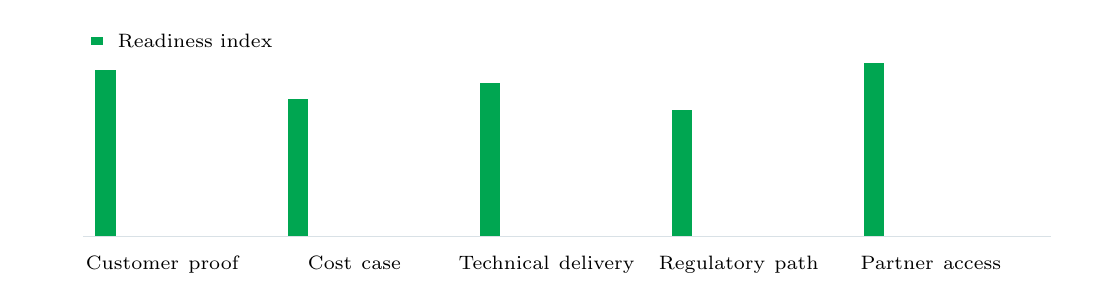
\begin{tikzpicture}[x=1cm,y=1cm]
\path[use as bounding box] (0,0) rectangle (13.20,3.20);
\draw[BOLine] (0.70,0.55) -- (13.00,0.55);
\fill[BOGreen] (0.86,0.55) rectangle (1.12,2.66);
\node[anchor=north,align=center,text width=2.24cm] at (1.71,0.42) {\scriptsize Customer proof};
\fill[BOGreen] (3.30,0.55) rectangle (3.56,2.29);
\node[anchor=north,align=center,text width=2.24cm] at (4.15,0.42) {\scriptsize Cost case};
\fill[BOGreen] (5.74,0.55) rectangle (6.00,2.50);
\node[anchor=north,align=center,text width=2.24cm] at (6.59,0.42) {\scriptsize Technical delivery};
\fill[BOGreen] (8.18,0.55) rectangle (8.44,2.16);
\node[anchor=north,align=center,text width=2.24cm] at (9.03,0.42) {\scriptsize Regulatory path};
\fill[BOGreen] (10.62,0.55) rectangle (10.88,2.75);
\node[anchor=north,align=center,text width=2.24cm] at (11.47,0.42) {\scriptsize Partner access};
\fill[BOGreen] (0.80,2.98) rectangle (0.96,3.08);
\node[anchor=west] at (1.02,3.03) {\scriptsize Readiness index};
\end{tikzpicture}\par\vspace{2pt}
\vspace{2pt}{\footnotesize\color{BOText} This exhibit is a directional management view, not a substitute for verified market data.}\par
{\scriptsize\color{BOMuted} BlueOcean public-source synthesis.}\par

\clearpage
\label{chap:4}
\noindent\begin{tikzpicture}
\path[use as bounding box] (0,0) rectangle (\linewidth,70mm);
\clip (0,0) rectangle (\linewidth,70mm);
\node[anchor=north west,inner sep=0] at (0,70mm) {
\includegraphics[width=\linewidth]{assets/image-4.png}};
\end{tikzpicture}
\vspace{0pt}
\noindent
\begin{tikzpicture}
\fill[BOGreen] (0,0) rectangle (96mm,1.2pt);
\end{tikzpicture}\par\vspace{8pt}
{\Large\sffamily\bfseries\color{BONavy} Strategic Implications Include Energy Independence and Reduced Fossil Fuel Leverage}\par\vspace{4pt}
{\sffamily\fontsize{16}{21}\selectfont\color{BOGreen} This chapter concludes that fusion could reshape global geopolitics by enabling energy independence and reducing fossil fuel leverage, but also poses nonproliferation risks and potential technology divides.}\par\vspace{11pt}
\begin{multicols}{2}
{\small Fusion energy has profound strategic implications for national security and global geopolitics. Countries that develop fusion technology could achieve near-total energy independence, reducing reliance on fossil fuel imports and insulating themselves from price volatility. This section explores the geopolitical dimensions of fusion commercialization.}\par
{\small Nations with active fusion programs include the United States, China, the European Union, Japan, South Korea, and Russia. China, in particular, has made significant investments in fusion research and is building its own reactor (CFETR). The ability to produce limitless clean energy could shift the balance of power, reducing the strategic importance of oil and gas reserves. OPEC nations and other fossil fuel exporters face a long-term existential threat to their revenue models.}\par
{\small However, fusion technology also raises nonproliferation risks. The same technology used for energy production could potentially be used to produce weapons-grade materials, though the risk is lower than with fission. International governance frameworks will be needed to ensure that fusion is used for peaceful purposes. The \BOApos{}fusion divide\BOApos{} between nations that have the technology and those that do not could exacerbate global inequalities.}\par
{\small For corporate strategists, the geopolitical implications mean that fusion investments should be evaluated not only on financial returns but also on strategic alignment with national energy security goals. Companies in energy-intensive industries may benefit from early access to fusion power, while those in fossil fuel sectors may need to diversify.}\par
\end{multicols}
\label{chap:4:end}

\clearpage
{\textcolor{BOGreen}{\scriptsize\bfseries EXHIBIT 7}}\par\vspace{3pt}
{\sffamily\fontsize{15}{19}\selectfont\color{BONavy} Commitment posture should shift as proof matures}\par
{\small\color{BOText} Resource posture for Nuclear Fusion Commercialization: Strategic Implications for Energy Markets and Investment}\par\vspace{4pt}
\noindent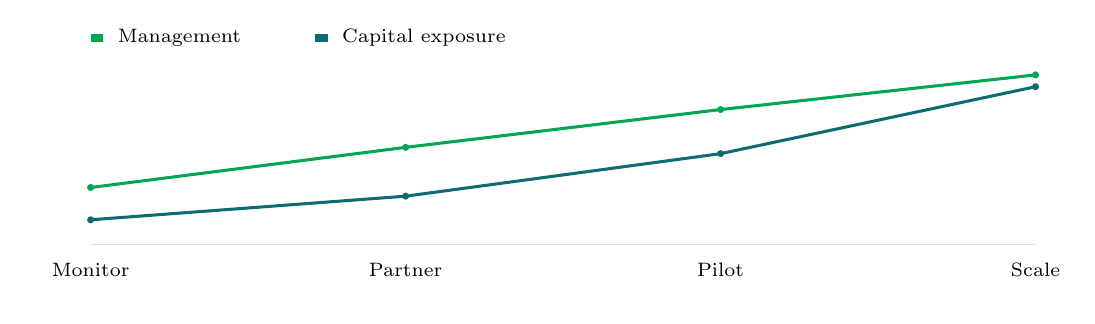
\begin{tikzpicture}[x=1cm,y=1cm]
\path[use as bounding box] (0,0) rectangle (13.20,3.40);
\draw[BOLine] (0.80,0.65) -- (12.80,0.65);
\draw[BOGreen,line width=1.1pt] (0.80,1.37) -- (4.80,1.88) -- (8.80,2.36) -- (12.80,2.80);
\fill[BOGreen] (0.80,1.37) circle (.045);
\fill[BOGreen] (4.80,1.88) circle (.045);
\fill[BOGreen] (8.80,2.36) circle (.045);
\fill[BOGreen] (12.80,2.80) circle (.045);
\draw[BOBlue,line width=1.1pt] (0.80,0.96) -- (4.80,1.26) -- (8.80,1.80) -- (12.80,2.65);
\fill[BOBlue] (0.80,0.96) circle (.045);
\fill[BOBlue] (4.80,1.26) circle (.045);
\fill[BOBlue] (8.80,1.80) circle (.045);
\fill[BOBlue] (12.80,2.65) circle (.045);
\node[anchor=north,align=center,text width=1.8cm] at (0.80,0.53) {\scriptsize Monitor};
\node[anchor=north,align=center,text width=1.8cm] at (4.80,0.53) {\scriptsize Partner};
\node[anchor=north,align=center,text width=1.8cm] at (8.80,0.53) {\scriptsize Pilot};
\node[anchor=north,align=center,text width=1.8cm] at (12.80,0.53) {\scriptsize Scale};
\fill[BOGreen] (0.80,3.22) rectangle (0.96,3.32);
\node[anchor=west] at (1.02,3.27) {\scriptsize Management};
\fill[BOBlue] (3.65,3.22) rectangle (3.81,3.32);
\node[anchor=west] at (3.87,3.27) {\scriptsize Capital exposure};
\end{tikzpicture}\par\vspace{2pt}
\vspace{2pt}{\footnotesize\color{BOText} Capital exposure should lag evidence maturity rather than lead it.}\par
{\scriptsize\color{BOMuted} BlueOcean scenario synthesis.}\par
\vspace{9pt}\textcolor{BOLine}{\rule{\linewidth}{0.3pt}}\vspace{8pt}
{\textcolor{BOGreen}{\scriptsize\bfseries EXHIBIT 8}}\par\vspace{3pt}
{\sffamily\fontsize{15}{19}\selectfont\color{BONavy} Key risks should be ranked by severity and manageability}\par
{\small\color{BOText} Risk exposure for Nuclear Fusion Commercialization: Strategic Implications for Energy Markets and Investment}\par\vspace{4pt}
\noindent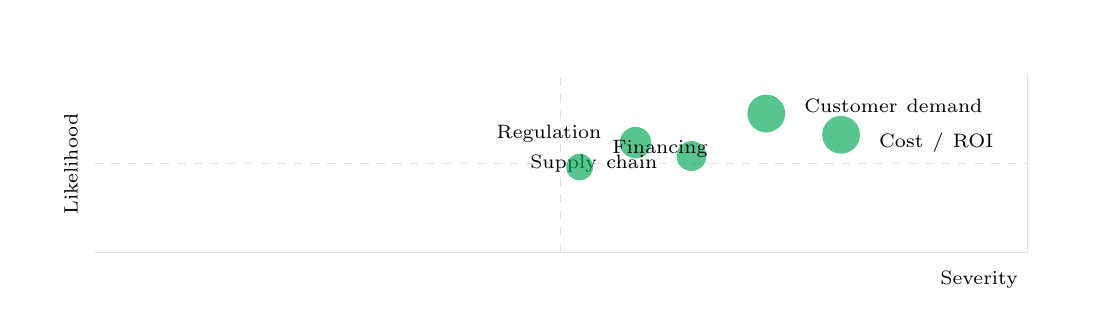
\begin{tikzpicture}[x=1cm,y=1cm]
\path[use as bounding box] (0,0) rectangle (13.20,3.50);
\draw[BOLine] (0.85,0.65) -- (12.70,0.65) -- (12.70,2.90);
\draw[BOLine,dashed] (0.85,1.77) -- (12.70,1.77);
\draw[BOLine,dashed] (6.77,0.65) -- (6.77,2.90);
\fill[BOGreen,opacity=.65] (9.38,2.41) circle (0.24);
\node[anchor=west,align=left,text width=2.45cm] at (9.74,2.51) {\scriptsize Customer demand};
\fill[BOGreen,opacity=.65] (10.33,2.14) circle (0.24);
\node[anchor=west,align=left,text width=2.45cm] at (10.69,2.04) {\scriptsize Cost / ROI};
\fill[BOGreen,opacity=.65] (7.72,2.04) circle (0.20);
\node[anchor=east,align=right,text width=2.45cm] at (7.41,2.15) {\scriptsize Regulation};
\fill[BOGreen,opacity=.65] (8.43,1.87) circle (0.19);
\node[anchor=east,align=right,text width=2.45cm] at (8.12,1.77) {\scriptsize Supply chain};
\fill[BOGreen,opacity=.65] (7.01,1.73) circle (0.17);
\node[anchor=west,align=left,text width=2.45cm] at (7.30,1.96) {\scriptsize Financing};
\node[anchor=north east] at (12.70,0.53) {\scriptsize Severity};
\node[anchor=center,rotate=90] at (0.55,1.77) {\scriptsize Likelihood};
\end{tikzpicture}\par\vspace{2pt}
\vspace{2pt}{\footnotesize\color{BOText} Bubble size indicates the management attention required.}\par
{\scriptsize\color{BOMuted} BlueOcean risk screen.}\par

\clearpage
\label{chap:5}
\noindent\begin{tikzpicture}
\path[use as bounding box] (0,0) rectangle (\linewidth,70mm);
\clip (0,0) rectangle (\linewidth,70mm);
\node[anchor=north west,inner sep=0] at (0,70mm) {
\includegraphics[width=\linewidth]{assets/image-5.png}};
\end{tikzpicture}
\vspace{0pt}
\noindent
\begin{tikzpicture}
\fill[BOGreen] (0,0) rectangle (96mm,1.2pt);
\end{tikzpicture}\par\vspace{8pt}
{\Large\sffamily\bfseries\color{BONavy} Investment Risks Are High but Early Movers May Gain Significant Advantage}\par\vspace{4pt}
{\sffamily\fontsize{16}{21}\selectfont\color{BOGreen} This chapter concludes that fusion investment carries substantial risks, but early movers can gain strategic advantages through staged, diversified approaches with clear milestones.}\par\vspace{11pt}
\begin{multicols}{2}
{\small Investing in fusion energy carries substantial risks, including technical, market, regulatory, and geopolitical uncertainties. However, the potential rewards for early movers could be enormous. This section provides a framework for assessing fusion investment opportunities.}\par
{\small The technical risk is the most significant: no fusion device has yet demonstrated sustained net energy gain. While private ventures like SPARC and Helion are making rapid progress, the history of fusion is filled with missed deadlines and unexpected challenges. Investors should be prepared for delays and setbacks.}\par
{\small Market risk is also substantial. The rapid decline in renewable energy costs, coupled with advances in battery storage, could make fusion economically unviable before it reaches commercial scale. Fusion\BOApos{}s competitiveness will depend on achieving low capital costs and high availability, which are unproven.}\par
{\small Regulatory and geopolitical risks add further uncertainty. The lack of a clear licensing framework could delay deployment, and the potential for technology divides or proliferation concerns could create political barriers. However, early movers who navigate these risks successfully could gain significant competitive advantages, including access to low-cost power, strategic partnerships, and intellectual property.}\par
\end{multicols}
\label{chap:5:end}

\clearpage
{\textcolor{BOGreen}{\scriptsize\bfseries EXHIBIT 9}}\par\vspace{3pt}
{\sffamily\fontsize{15}{19}\selectfont\color{BONavy} Diligence workload concentrates in customer, cost and policy proof}\par
{\small\color{BOText} Near-term validation load for Nuclear Fusion Commercialization: Strategic Implications for Energy Markets and Investment}\par\vspace{4pt}
\noindent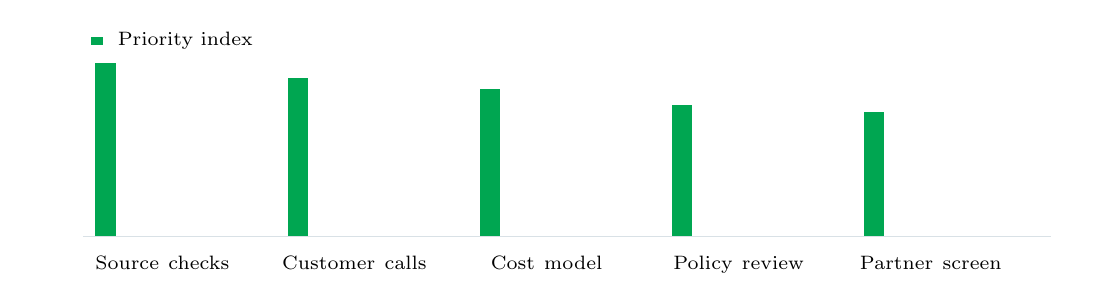
\begin{tikzpicture}[x=1cm,y=1cm]
\path[use as bounding box] (0,0) rectangle (13.20,3.20);
\draw[BOLine] (0.70,0.55) -- (13.00,0.55);
\fill[BOGreen] (0.86,0.55) rectangle (1.12,2.75);
\node[anchor=north,align=center,text width=2.24cm] at (1.71,0.42) {\scriptsize Source checks};
\fill[BOGreen] (3.30,0.55) rectangle (3.56,2.56);
\node[anchor=north,align=center,text width=2.24cm] at (4.15,0.42) {\scriptsize Customer calls};
\fill[BOGreen] (5.74,0.55) rectangle (6.00,2.42);
\node[anchor=north,align=center,text width=2.24cm] at (6.59,0.42) {\scriptsize Cost model};
\fill[BOGreen] (8.18,0.55) rectangle (8.44,2.22);
\node[anchor=north,align=center,text width=2.24cm] at (9.03,0.42) {\scriptsize Policy review};
\fill[BOGreen] (10.62,0.55) rectangle (10.88,2.13);
\node[anchor=north,align=center,text width=2.24cm] at (11.47,0.42) {\scriptsize Partner screen};
\fill[BOGreen] (0.80,2.98) rectangle (0.96,3.08);
\node[anchor=west] at (1.02,3.03) {\scriptsize Priority index};
\end{tikzpicture}\par\vspace{2pt}
\vspace{2pt}{\footnotesize\color{BOText} The most valuable work closes open questions that can change the decision.}\par
{\scriptsize\color{BOMuted} BlueOcean public-source synthesis.}\par
\vspace{9pt}\textcolor{BOLine}{\rule{\linewidth}{0.3pt}}\vspace{8pt}
{\textcolor{BOGreen}{\scriptsize\bfseries EXHIBIT 10}}\par\vspace{3pt}
{\sffamily\fontsize{15}{19}\selectfont\color{BONavy} Scenario choices should compare attractiveness with readiness}\par
{\small\color{BOText} Strategic option comparison for Nuclear Fusion Commercialization: Strategic Implications for Energy Markets and Investment}\par\vspace{4pt}
{\scriptsize\begin{tabular}{p{38mm}>{\centering\arraybackslash}p{21mm}>{\centering\arraybackslash}p{21mm}>{\centering\arraybackslash}p{21mm}>{\centering\arraybackslash}p{21mm}}
 & {\bfseries Attractiveness} & {\bfseries Readiness} & {\bfseries Evidence quality} & {\bfseries Capital need} \\
\hline
{\bfseries Fusion Commercialization Is} & \colorbox{BOGreen}{\textcolor{white}{\strut\hspace{5pt}5\hspace{5pt}}} & \colorbox{BOBlue}{\textcolor{white}{\strut\hspace{5pt}3\hspace{5pt}}} & \colorbox{BOLight}{\textcolor{BOText}{\strut\hspace{5pt}2\hspace{5pt}}} & \colorbox{BOLight}{\textcolor{BOText}{\strut\hspace{5pt}2\hspace{5pt}}} \\
{\bfseries Private Ventures Are Outpacing} & \colorbox{BOGreen}{\textcolor{white}{\strut\hspace{5pt}4\hspace{5pt}}} & \colorbox{BOGreen}{\textcolor{white}{\strut\hspace{5pt}4\hspace{5pt}}} & \colorbox{BOBlue}{\textcolor{white}{\strut\hspace{5pt}3\hspace{5pt}}} & \colorbox{BOBlue}{\textcolor{white}{\strut\hspace{5pt}3\hspace{5pt}}} \\
{\bfseries Economic Viability Remains} & \colorbox{BOGreen}{\textcolor{white}{\strut\hspace{5pt}4\hspace{5pt}}} & \colorbox{BOLight}{\textcolor{BOText}{\strut\hspace{5pt}2\hspace{5pt}}} & \colorbox{BOLight}{\textcolor{BOText}{\strut\hspace{5pt}2\hspace{5pt}}} & \colorbox{BOGreen}{\textcolor{white}{\strut\hspace{5pt}4\hspace{5pt}}} \\
{\bfseries Strategic Implications Include} & \colorbox{BOBlue}{\textcolor{white}{\strut\hspace{5pt}3\hspace{5pt}}} & \colorbox{BOBlue}{\textcolor{white}{\strut\hspace{5pt}3\hspace{5pt}}} & \colorbox{BOBlue}{\textcolor{white}{\strut\hspace{5pt}3\hspace{5pt}}} & \colorbox{BOLight}{\textcolor{BOText}{\strut\hspace{5pt}2\hspace{5pt}}} \\
{\bfseries Investment Risks Are High} & \colorbox{BOGreen}{\textcolor{white}{\strut\hspace{5pt}5\hspace{5pt}}} & \colorbox{BOBlue}{\textcolor{white}{\strut\hspace{5pt}3\hspace{5pt}}} & \colorbox{BOBlue}{\textcolor{white}{\strut\hspace{5pt}3\hspace{5pt}}} & \colorbox{BOBlue}{\textcolor{white}{\strut\hspace{5pt}3\hspace{5pt}}} \\
\end{tabular}}\par\vspace{2pt}
\vspace{2pt}{\footnotesize\color{BOText} The matrix ranks where the next validation work should focus.}\par
{\scriptsize\color{BOMuted} BlueOcean qualitative assessment.}\par

\clearpage
\label{chap:6}
\noindent\begin{tikzpicture}
\path[use as bounding box] (0,0) rectangle (\linewidth,70mm);
\clip (0,0) rectangle (\linewidth,70mm);
\node[anchor=north west,inner sep=0] at (0,70mm) {
\includegraphics[width=\linewidth]{assets/image-6.png}};
\end{tikzpicture}
\vspace{0pt}
\noindent
\begin{tikzpicture}
\fill[BOGreen] (0,0) rectangle (96mm,1.2pt);
\end{tikzpicture}\par\vspace{8pt}
{\Large\sffamily\bfseries\color{BONavy} Nuclear Fusion Commercialization: Strategic Implications for Energy Markets and Investment should be managed as a staged strategic option, not a binary bet}\par\vspace{4pt}
{\sffamily\fontsize{16}{21}\selectfont\color{BOGreen} The CEO question is which moves are safe now and which should wait for stronger evidence.}\par\vspace{11pt}
\begin{multicols}{2}
{\small For leadership, Nuclear Fusion Commercialization: Strategic Implications for Energy Markets and Investment should be separated into verified facts, directional scenarios and open diligence items. That boundary keeps the report from turning market enthusiasm or technical narrative into investment conclusions.}\par
{\small The immediate management question is not whether the opportunity is exciting; it is whether budget, partner access or management attention should be committed now. Low-cost validation can start early, while larger capital commitments should wait for customer, cost, financing, regulatory or operating proof.}\par
{\small The current evidence posture is: Public evidence retained in the supporting sources; additional validation is required for unsupported claims. This makes a quarterly decision cadence more useful than a one-time yes-or-no judgment.}\par
\end{multicols}
\label{chap:6:end}

\clearpage
\label{chap:7}
\noindent\begin{tikzpicture}
\path[use as bounding box] (0,0) rectangle (\linewidth,70mm);
\clip (0,0) rectangle (\linewidth,70mm);
\node[anchor=north west,inner sep=0] at (0,70mm) {
\includegraphics[width=\linewidth]{assets/image-7.png}};
\end{tikzpicture}
\vspace{0pt}
\noindent
\begin{tikzpicture}
\fill[BOGreen] (0,0) rectangle (96mm,1.2pt);
\end{tikzpicture}\par\vspace{8pt}
{\Large\sffamily\bfseries\color{BONavy} Commercial readiness depends on bankability, deliverability and repeat customer proof}\par\vspace{4pt}
{\sffamily\fontsize{16}{21}\selectfont\color{BOGreen} Technical feasibility matters only when it changes customer value, cost position and execution confidence.}\par\vspace{11pt}
\begin{multicols}{2}
{\small Commercial readiness should be judged through customer adoption, cost structure, delivery cycle, service capability and financing availability. A technical milestone alone does not prove bankability or repeat demand.}\par
{\small Management should require every major assumption to tie back to a verifiable claim: target customer, buying trigger, budget owner, substitute, use case and payback path. Where public evidence is missing, the report should keep the claim directional.}\par
{\small A more robust path is to build credible proof through pilots, partner diligence and third-party validation before moving into larger commitments.}\par
\end{multicols}
\label{chap:7:end}

\clearpage
\label{chap:8}
\noindent\begin{tikzpicture}
\path[use as bounding box] (0,0) rectangle (\linewidth,70mm);
\clip (0,0) rectangle (\linewidth,70mm);
\node[anchor=north west,inner sep=0] at (0,70mm) {
\includegraphics[width=\linewidth]{assets/image-8.png}};
\end{tikzpicture}
\vspace{0pt}
\noindent
\begin{tikzpicture}
\fill[BOGreen] (0,0) rectangle (96mm,1.2pt);
\end{tikzpicture}\par\vspace{8pt}
{\Large\sffamily\bfseries\color{BONavy} Cost, return and timing will determine the real deployment window}\par\vspace{4pt}
{\sffamily\fontsize{16}{21}\selectfont\color{BOGreen} Market size should not enter an investment case until the cost and return logic can be checked.}\par\vspace{11pt}
\begin{multicols}{2}
{\small Every opportunity eventually returns to cost, revenue, margin, cash flow and timing. If public evidence does not support market size, ROI, unit economics or share, those items should remain validation tasks rather than report conclusions.}\par
{\small Near-term action should focus on verifiable cost drivers and customer willingness to pay instead of relying on optimistic long-range scenarios. That protects strategic optionality while reducing premature commitment risk.}\par
{\small As cost, customer and financing evidence improves, management can shift resources from monitoring and partnerships toward pilots or scaled deployment.}\par
\end{multicols}
\label{chap:8:end}

\clearpage
{\sffamily\fontsize{20}{25}\selectfont\color{BONavy} About the research}\par\vspace{6pt}
\vspace{2pt}{\color{BOBright}\rule{\linewidth}{1pt}}\vspace{5pt}
{\footnotesize\color{BOMuted} This report has been prepared for strategy discussion and executive decision support. It is not investment, legal, tax, audit or valuation advice. Market estimates, forecasts and scenarios are directional and should be independently validated before they are used for investment, financing, transaction, regulatory or operational decisions. Forward-looking views may change as technology, policy, financing, regulation, competition, supply chains and macro conditions evolve. Recipients should perform their own diligence and treat this report as one input into a broader decision process.}


\clearpage
\thispagestyle{empty}
\begin{tikzpicture}[remember picture,overlay]
\node[anchor=south west,inner sep=0] at (current page.south west) {
\includegraphics[width=\paperwidth,height=\paperheight]{assets/cover-ai.png}};
\fill[black,opacity=.45] (current page.south west) rectangle (current page.north east);
\node[anchor=south east] at ([xshift=-11mm,yshift=10mm]current page.south east) {\sffamily\bfseries\Large\color{white} BlueOcean};
\end{tikzpicture}

\end{document}
